% =====================================================================
%  CHAPTER 3 — SYSTEM REQUIREMENTS AND ANALYSIS
% =====================================================================
\clearpage
\chapter{System Requirements and Analysis}

This chapter derives the requirements the engine must satisfy, specifies the
software and hardware environment in which it is built and measured, and
records the assumptions and constraints under which the design in Chapter~4
was made. Requirements are stated so that each is testable: a requirement that
cannot be checked by an automated assertion against a running cluster has been
reformulated until it can be.

\section{Functional Requirements}

The functional requirements fall into six groups, corresponding to the six
mechanisms the engine implements. Tables~\ref{tab:funcreq}
and~\ref{tab:funcreq2} list them with the identifier used throughout the
remainder of the report.

\begin{table}[htbp]
  \centering
  \caption{Functional requirements}
  \label{tab:funcreq}
  \small
  \begin{tabular}{@{}p{0.42in}p{2.3in}p{1.98in}@{}}
    \toprule
    \textbf{ID} & \textbf{Requirement} & \textbf{Verified by} \\
    \midrule
    FR-1 & Every workflow state transition shall be persisted as an immutable
      event before it is acted upon &
      Assert no \cd{UPDATE} or \cd{DELETE} is ever issued against the event log \\
    FR-2 & A workflow interrupted at any point shall resume from its recorded
      history without re-executing completed activities &
      Kill a node mid-workflow; compare completed-activity counts before and
      after \\
    FR-3 & The engine shall detect and refuse to continue a workflow whose code
      takes a different branch on replay &
      Inject a deliberate non-determinism; assert the workflow fails loudly \\
    FR-4 & A failed activity shall be retried according to a configurable
      policy with exponential backoff &
      An activity failing three times then succeeding shall produce exactly one
      success event \\
    FR-5 & The engine shall supply each activity with a deduplication key that
      is stable across crashes and replays &
      Assert the key observed by the activity is identical on every attempt \\
    FR-6 & Workflow execution shall be partitioned across a fixed number of
      shards, and each workflow shall remain in one shard for its lifetime &
      Assert shard assignment is unchanged across the full life of 1{,}000
      workflows \\
    FR-7 & Shard ownership shall transfer automatically when the owning node
      fails &
      Kill the owner; assert another node acquires the lease and resumes work \\
    FR-8 & A node that has lost ownership shall be unable to commit any change
      to that shard &
      Freeze a node past its lease expiry; assert its transaction rolls back \\
    FR-9 & Adding or removing a node shall move ownership of a minority of
      shards and migrate no workflow data &
      Add a fourth node to a three-node cluster; count reassigned shards \\
    \bottomrule
  \end{tabular}
\end{table}

\begin{table}[htbp]
  \centering
  \caption{Functional requirements (continued)}
  \label{tab:funcreq2}
  \small
  \begin{tabular}{@{}p{0.42in}p{2.3in}p{1.98in}@{}}
    \toprule
    \textbf{ID} & \textbf{Requirement} & \textbf{Verified by} \\
    \midrule
    FR-10 & A workflow shall be able to sleep for an arbitrary duration without
      holding a thread, connection or memory &
      Start a workflow with a two-minute sleep; restart the whole cluster;
      assert it wakes on schedule \\
    FR-11 & An external signal shall be durable before any workflow code
      observes it &
      Send a signal and kill the cluster immediately; assert the signal survives \\
    FR-12 & A multi-step transaction failing partway shall run compensations
      for completed steps in reverse order &
      Force a late step to fail; assert compensation events appear in LIFO
      order \\
    FR-13 & A compensation that exhausts its retries shall leave the workflow in
      a distinct terminal state requiring human intervention &
      Assert status \cd{COMPENSATING\_FAILED} is reachable and surfaced \\
    FR-14 & For activities configured in semantic mode, a semantically
      equivalent repeated action shall be suppressed before it executes &
      Count real side effects in an external ledger across an induced agent
      re-plan \\
    FR-15 & Every deduplication verdict shall be journalled with its similarity
      score, threshold and matched predecessor &
      Assert the verdict event is present and queryable through the API \\
    FR-16 & The engine shall expose workflow start, query, history retrieval,
      signalling and cancellation over HTTP &
      Contract tests against each documented endpoint \\
    FR-17 & The engine shall export metrics suitable for a time-series database
      & Scrape \cd{/metrics} and assert the expected series exist \\
    FR-18 & The engine shall provide a fault-injection facility that crashes a
      node at a named point in the execution path &
      Assert each named crash point is reachable and produces the documented
      state \\
    \bottomrule
  \end{tabular}
\end{table}

Two of these deserve comment because they are unusual as requirements.

FR-3 requires the engine to \emph{fail} rather than to recover. When replay
produces a different sequence of decisions from the original execution, the
engine cannot know which version of the code told the truth, and any attempt
to reconcile the two would silently corrupt the history. Refusing to continue
is the only safe behaviour, and detecting the condition at all is a
non-trivial design obligation discharged in Section~4.2.3.

FR-8 is the central safety requirement of the whole system and is stated in
the negative deliberately. It is not enough that ownership transfers; it must
additionally be impossible for the previous owner to act, even though that
node has no way of knowing it has been displaced. Section~4.1.5 gives the
mechanism.

\section{Non-Functional Requirements}

\begin{table}[htbp]
  \centering
  \caption{Non-functional requirements}
  \label{tab:nonfuncreq}
  \small
  \begin{tabular}{@{}p{0.45in}p{1.2in}p{2.92in}@{}}
    \toprule
    \textbf{ID} & \textbf{Attribute} & \textbf{Requirement} \\
    \midrule
    NFR-1 & Correctness &
      Zero committed work shall be lost under induced node failure. This is an
      absolute requirement, not a target. \\
    NFR-2 & Correctness &
      Zero activities shall execute twice as a result of a failover, excluding
      the irreducible crash window of Section~4.2.8. \\
    NFR-3 & Availability &
      A shard shall be unavailable for at most the lease duration following the
      loss of its owner. With the default ten-second lease this bounds
      unavailability to ten seconds for $1/N$ of workflows. \\
    NFR-4 & Scalability &
      Throughput shall increase materially when shard count is doubled; the
      scaling ratio, not the absolute rate, is the reported figure. \\
    NFR-5 & Latency &
      Reconstructing a workflow's state from a two-hundred-event history shall
      complete in under fifty milliseconds at the 99th percentile. \\
    NFR-6 & Operability &
      The system shall require exactly one infrastructure dependency. No message
      broker, coordination service or search index may be introduced. \\
    NFR-7 & Portability &
      A node shall be a single statically linked binary, deployable as a
      container image without a runtime interpreter. \\
    NFR-8 & Observability &
      Every failover, retry, compensation and deduplication verdict shall be
      visible as a metric or as a queryable event. \\
    NFR-9 & Resource footprint &
      The complete demonstration cluster shall run within the memory of a single
      developer workstation. \\
    NFR-10 & Auditability &
      Any suppressed side effect shall be explainable from stored data alone,
      without re-running any model. \\
    NFR-11 & Security &
      No component intended for testing shall be reachable from outside the
      host, and no credential shall appear in source control. \\
    \bottomrule
  \end{tabular}
\end{table}

NFR-6 is a constraint rather than a goal, and it is the one that most shapes
Chapter~4. Several otherwise attractive designs --- a Redis-backed task queue,
a Kafka-backed event log, a ZooKeeper-based ownership service --- are excluded
by it. The justification is the argument of Section~1.2.1: for the deployment
scale this project targets, each additional component costs more in
operational risk than it returns in capability.

NFR-9 deserves a candid note. The demonstration cluster was sized to fit a
single workstation because that is the hardware available, and this constrains
what the evaluation can claim. It does not constrain correctness results ---
whether work was lost or duplicated is independent of how fast the machine is
--- but it does mean that absolute throughput figures from this project are
not comparable with figures from systems evaluated in data centres. This is
restated in Section~3.5 as an explicit constraint on the evaluation.

\section{Software Requirements}

\begin{table}[htbp]
  \centering
  \caption{Software requirements}
  \label{tab:swreq}
  \small
  \begin{tabular}{@{}p{1.22in}p{0.85in}p{2.5in}@{}}
    \toprule
    \textbf{Component} & \textbf{Version} & \textbf{Role and justification} \\
    \midrule
    Go & 1.25.10 &
      Implementation language. Chosen for goroutines, which make the
      cooperative scheduler of Section~4.2.4 expressible, and for static
      linking, which satisfies NFR-7. \\
    PostgreSQL & 16 &
      The sole infrastructure dependency. Supplies the event log, the task
      queue, the timer store and the ownership record. Chosen for
      \cd{SKIP LOCKED}, \cd{FOR UPDATE} and streaming replication. \\
    pgvector extension & bundled in the container image &
      Stores 384-dimensional embeddings for the semantic idempotency
      comparator. \\
    jackc/pgx & v5.10.0 &
      PostgreSQL driver and connection pool. Chosen over \cd{database/sql} for
      native protocol support and explicit pool statistics. \\
    Docker Engine and Compose & current stable &
      Reproducible multi-node deployment on one host. \\
    Prometheus & v2.55.1 & Metrics collection, satisfying NFR-8. \\
    Grafana & 11.2.0 & Dashboards over the collected metrics. \\
    client\_golang & v1.24.1 &
      Metric instrumentation inside the engine binary. \\
    \cd{all-MiniLM-L6-v2} & --- &
      The sentence-embedding model behind the semantic comparator. Chosen for
      its small size and 384-dimensional output, which keeps the vector column
      narrow. \\
    \bottomrule
  \end{tabular}
\end{table}

Three choices in Table~\ref{tab:swreq} were contested during design and are
justified here rather than left implicit.

\textbf{Go rather than Java or Rust.} The workflow dispatcher of
Section~4.2.4 requires a construct that can suspend a function mid-execution
and resume it later under the engine's control rather than the operating
system's. Go's goroutines and unbuffered channels express this handshake in a
few lines. Java would require either threads, which are too heavy for one per
in-flight workflow, or a bytecode-level continuation library. Rust's
\cd{async} machinery would work but introduces lifetime complexity
disproportionate to the benefit at this scale.

\textbf{PostgreSQL rather than a key-value store.} The engine's correctness
rests on committing a workflow decision and all of its consequences --- new
events, new task rows, new timer rows, an updated execution pointer --- in a
single atomic transaction. A key-value store without multi-key transactions
would require the engine to implement that atomicity itself, which is
precisely the complexity the design is trying to remove.

\textbf{A relational table rather than a dedicated queue.} \cd{FOR UPDATE SKIP
LOCKED} allows many workers to poll the same table concurrently without
serialising behind one another, which is the property that makes an external
broker unnecessary. Section~4.2.6 gives the query and explains why the clause
is load-bearing rather than an optimisation.

\section{Hardware Requirements}

This is a software project; the hardware requirement is that of the
development and measurement environment rather than of a manufactured
artefact. Table~\ref{tab:hwreq} records it, and Fig.~\ref{fig:testbench} shows
the topology that runs on it.

\begin{table}[htbp]
  \centering
  \caption{Hardware requirements of the development and measurement
    environment}
  \label{tab:hwreq}
  \small
  \begin{tabular}{@{}p{1.25in}p{1.3in}p{1.92in}@{}}
    \toprule
    \textbf{Resource} & \textbf{Minimum} & \textbf{Rationale} \\
    \midrule
    Processor & 4 cores, x86-64 &
      Three engine containers plus two PostgreSQL instances plus the
      observability stack must run concurrently without the measurement
      competing with the system being measured. \\
    Memory & 8\,GB usable &
      The base stack occupies approximately 2.3\,GB; adding the embedding model
      raises this to approximately 3.2\,GB. \\
    Storage & 20\,GB free &
      Container images, two PostgreSQL data directories, and an event log that
      has no garbage collection. \\
    Network & Loopback only &
      The entire cluster runs on one host; no component is exposed beyond it,
      satisfying NFR-11. \\
    Accelerator & None required &
      The embedding model runs acceptably on CPU for the candidate-set sizes
      involved, which are tens of vectors rather than millions. \\
    \bottomrule
  \end{tabular}
\end{table}

\begin{figure}[htbp]
  \centering
  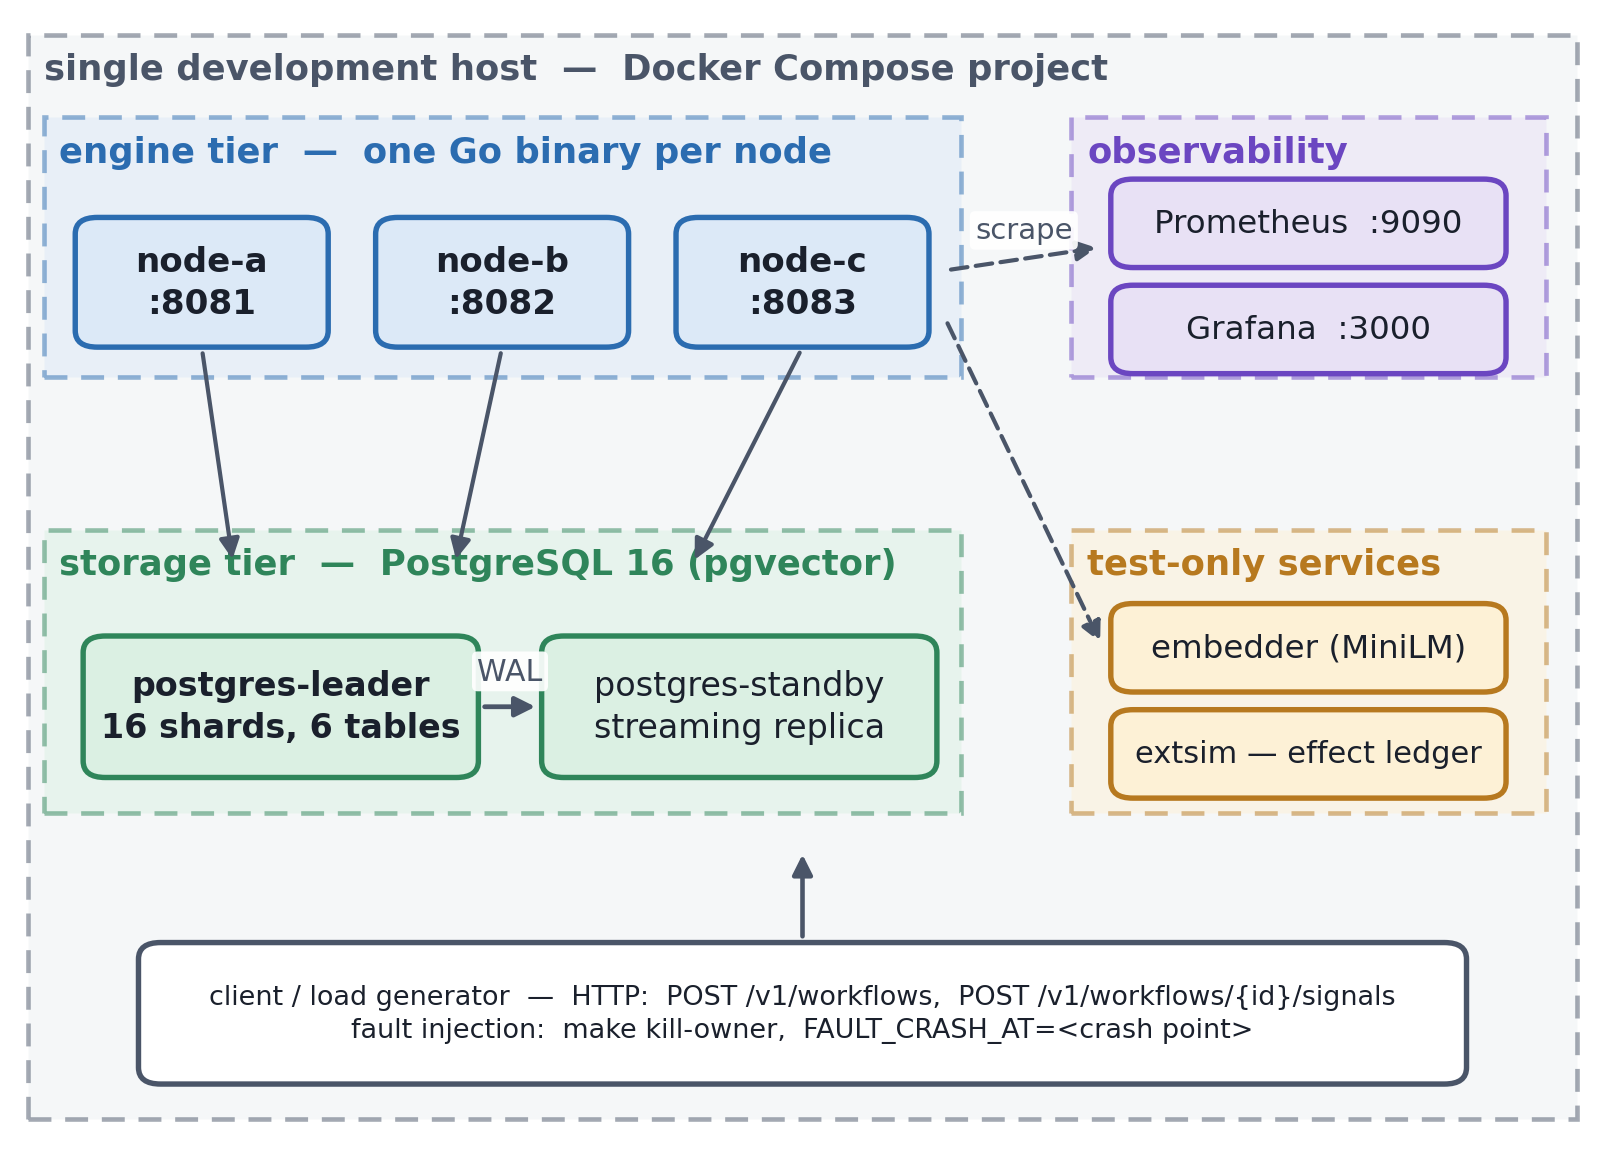
\includegraphics[width=\linewidth]{figures/fig_3_1_testbench.png}
  \caption{The container topology against which the requirements of this
    chapter are sized, and on which every measurement reported by this project
    was taken. Three engine nodes share one PostgreSQL leader with a streaming
    standby; the embedder and the external-effect simulator are test-only
    services and are never exposed beyond the host.}
  \label{fig:testbench}
\end{figure}

\section{Assumptions and Constraints}

\begin{table}[htbp]
  \centering
  \caption{Assumptions and constraints under which the design was made}
  \label{tab:assumptions}
  \small
  \begin{tabular}{@{}p{0.45in}p{1.05in}p{3.07in}@{}}
    \toprule
    \textbf{ID} & \textbf{Type} & \textbf{Statement} \\
    \midrule
    A-1 & Assumption &
      PostgreSQL provides linearizable reads and writes for a single row under
      \cd{FOR UPDATE}. The entire ownership-safety argument depends on this and
      on nothing else. \\
    A-2 & Assumption &
      Workflow authors write deterministic orchestration code. The engine
      detects violations (FR-3) but cannot repair them. \\
    A-3 & Assumption &
      Clocks on different nodes may disagree, but each node's view of elapsed
      time is monotonic. Lease expiry is evaluated by the database, not by the
      nodes, specifically so that cross-node clock skew cannot affect
      correctness. \\
    A-4 & Assumption &
      Downstream services honour an idempotency key when one is supplied. The
      irreducible crash window of Section~4.2.8 can only be closed by the
      resource itself. \\
    C-1 & Constraint &
      Exactly one infrastructure dependency is permitted (NFR-6). \\
    C-2 & Constraint &
      Evaluation hardware is a single workstation. Absolute throughput is
      therefore not comparable with published data-centre figures; scaling
      ratios and correctness counts are. \\
    C-3 & Constraint &
      Ownership uses lease renewal backed by a linearizable database rather than
      a full consensus protocol. This is a deliberate scope decision recorded in
      Section~1.5. \\
    C-4 & Constraint &
      The semantic comparator must not be consulted during replay, because
      recovery may not depend on the availability of an external model. This
      constraint dictates the design of Section~4.2.10 almost entirely. \\
    C-5 & Constraint &
      No credential may be committed to source control, and no test-only service
      may be reachable from outside the host. \\
    \bottomrule
  \end{tabular}
\end{table}

Assumption A-3 is worth expanding, because clock handling is where lease-based
systems most often go wrong. The engine never compares a timestamp generated
on one node against a timestamp generated on another. Lease expiry is expressed
as \cd{expires\_at < now()} and evaluated inside the database, so all
comparisons occur against a single clock. A node whose own clock is badly wrong
will renew its lease too eagerly or too lazily, but it cannot cause two nodes
to believe simultaneously that they own the same shard, because the decision is
made in one place.

\section{Analysis of the Chosen Approach}

The requirements above admit several architectures. Table~\ref{tab:stack}
records the principal alternatives considered and the reason each was rejected,
so that the design presented in Chapter~4 is understood as a choice among
options rather than as the only possibility.

\begin{table}[htbp]
  \centering
  \caption{Architectural alternatives considered and reasons for rejection}
  \label{tab:stack}
  \small
  \begin{tabular}{@{}p{1.15in}p{1.52in}p{1.98in}@{}}
    \toprule
    \textbf{Alternative} & \textbf{Attraction} & \textbf{Reason rejected} \\
    \midrule
    Build on Temporal or Restate &
      Mature, production-proven, saves months &
      The project \emph{is} the implementation; and the semantic idempotency
      contribution requires modifying the engine's decision path, which cannot
      be done from outside as a user of the platform \\
    Kafka as the event log &
      Purpose-built append-only log with replication &
      Violates NFR-6; and a workflow decision plus its task and timer rows
      could no longer be committed atomically with the events \\
    Redis or RabbitMQ task queue &
      Lower polling latency than a database table &
      Violates NFR-6; \cd{SKIP LOCKED} already provides concurrent
      non-blocking dequeue within the existing dependency \\
    ZooKeeper or etcd for ownership &
      The textbook answer, used by Shard Manager~\cite{shardmanager2021} &
      Violates NFR-6; a fencing token re-checked inside the write transaction
      provides the same safety property (Section~4.1.5) \\
    Full Raft for ownership &
      True consensus, with no reliance on a single database &
      Disproportionate to the scale targeted; recorded as future work in
      Section~1.5 \\
    One database per shard &
      Removes the shared-database bottleneck &
      Every key already carries the shard identifier, so this is a deployment
      change; deferred rather than rejected \\
    Single-node design, as in DBOS~\cite{dbos2025} &
      Far simpler; no ownership problem at all &
      Objective~4 requires horizontal partitioning, which is precisely the
      aspect DBOS does not address \\
    Lock-based rollback instead of sagas &
      Stronger isolation between concurrent workflows &
      Measured by AC/DC~\cite{acdc2026} to fail 42\% of orders at one-second
      steps; compensation is the empirically supported choice \\
    \bottomrule
  \end{tabular}
\end{table}

The resulting position can be summarised in one sentence: \textbf{the engine
keeps the single-dependency simplicity of the DBOS line of work while adding
the horizontal partitioning that line does not attempt, and it obtains the
ownership safety that normally justifies a coordination service from a fencing
token re-checked inside each write transaction.} Chapter~4 develops that
position into a complete design.
